\documentclass[a4paper, 12pt]{article}

% english
\usepackage[english]{babel}
\usepackage{lmodern}

% biblio
%\usepackage{csquotes}
%\usepackage[backend=biber, language=english]{biblatex}
%\addbibresource{./biblio.bib}

% packages
\usepackage{fullpage}				% really narrow margins
\usepackage{graphicx}				% \includegraphics
\usepackage{amsmath}				% \text
\usepackage{amsfonts}				% \mathbb
\usepackage{multirow}				% \multirow		
\usepackage{enumitem}				% \setitemsize
\usepackage{appendix}				% appendix env
\usepackage{pgf, tikz}			% figures

% center vertically
\usepackage{titling}				
\renewcommand\maketitlehooka{\null\mbox{}\vfill}
\renewcommand\maketitlehookd{\vfill\null}

% figures
\usetikzlibrary{positioning}

% misc
\addto\captionsenglish{\def\chaptername{Part}}		% Part/Chapter
\renewcommand\thesection{\arabic{section}}				% arabic numbers
\setlength\parindent{0pt}													% no indentation
\setitemize{itemsep=0em}													% no space between itms

% algorithms
\usepackage{algpseudocode}
\usepackage[linesnumbered, ruled]{algorithm2e}
\usepackage{stmaryrd}

 %code (default C++)
\usepackage{listings}
\usepackage{xcolor}
\definecolor{keyword}{rgb}{0.76,0.18,0.64}
\definecolor{directive}{rgb}{0.47,0.28,0.18}
\definecolor{string}{rgb}{0.85,0.16,0.14}
\definecolor{comment}{rgb}{0.43,0.65,0.38}
\lstdefinestyle{cpp}{
  language=C++,
  tabsize=2,
  keepspaces=true,
  showspaces=false,
  showtabs=false,
  showstringspaces=false,
  basicstyle=\ttfamily\footnotesize,
  keywordstyle=\color{keyword}\ttfamily,
  stringstyle=\color{string}\ttfamily,
  commentstyle=\color{comment}\ttfamily,
  morecomment=[l][\color{directive}]{\#}
}
%\lstdefinestyle{xml}{
%  language=C++,
%  tabsize=2,
%  keepspaces=true,
%  showspaces=false,
%  showtabs=false,
%  showstringspaces=false,
%  basicstyle=\ttfamily\footnotesize,
%  stringstyle=\color{string},
%  identifierstyle=\color{directive},
%  keywordstyle=\color{directive},
%  morestring=[b]",
%  moredelim=[s]{>}{<},
%  morecomment=[s]{<?}{?>},
%  morekeywords={} % list attr here
%}


\title{Computer Science}
\date{}

\begin{document}

%\begin{titlingpage}
\maketitle
%\end{titlingpage}

%\newpage
\tableofcontents
%\listoffigures
%\newpage



%\addcontentsline{toc}{section}{References}
%\printbibliography

\section{Master Theorem}

\noindent For recurrences of the form $T(n) = aT(\frac{n}{b}) + f(n)$, where:
\begin{itemize}
  \item $a\ge 1$ and $b>1$ are constants
  \item $f(n)$ is an asymptotically positive function
\end{itemize}
\begin{enumerate}
  \item If $f(n) = O(n^{\log_b(a)-\epsilon})$ for some constant $\epsilon >0$, then $T(n) = \Theta(n^{\log_b(a)})$.
  \item Either of the following:\\
    If $f(n) = \Theta(n^{\log_b(a)})$, then $T(n) = \Theta(n^{\log_b(a)}\log(n))$.\\
    If $f(n) = \Theta(n^{\log_b(a)}\log^k(n))$, then $T(n) = \Theta(n^{\log_b^{k+1}(a)}\log(n))$.
  \item If $f(n) = \Omega(n^{\log_b(a)+\epsilon})$ for some constant $\epsilon >0$, and if $af(\frac{n}{b})\le cf(n)$ for some constant $c<1$ and all sufficiently large $n$, then $T(n) = \Theta(f(n))$.
\end{enumerate}

\section{NP-Completeness}

  \subsection{Definition}

A problem is NP-Complete if it is both:
\begin{itemize}
  \item In NP: can be solvable in polynomial time on a non-deterministic Turing machine, or which can be verified in polynomial time.
  \item NP-hard: any problem in NP can be reduced in polynomial time to this problem.
\end{itemize}

  \subsection{Reducibility}

A language $L_1$ is polynomial-time reducible to a language $L_2$, written $L_1\le _PL_2$, if there exists a polynomial-time computable function $f$ such that for all $x$, $x\in L_1\Leftrightarrow f(x)\in L_2$.

  \subsection{Proof of NP-Completeness}

If $L$ is a language such that $L'\le_PL$ for some $L'\in$ NPC, then $L$ is NP-hard. If, in addition, $L\in$ NP, then $L\in$ NPC.
In other words, to show that a language is NP-complete:
\begin{enumerate}
  \item Show that $L\in$ NP (CLIQUE).
  \item Select a known NP-complete language $L'$ (SAT).
  \item Find $f$ mapping every instance of $L'$ to an instance of $L$ (SAT $\le_P$ CLIQUE).
  \item Prove that $x\in L'\Leftrightarrow f(x)\in L$ and $f$ runs in polynomial-time.
\end{enumerate}

\section{Basic Maths}

  \subsection{Series}

$$\sum_{i=0}^{n}i = \frac{n(n+1)}{2}$$
$$\sum_{i=0}^{n}i^2 = \frac{n(n+1)(2n+1)}{6}$$
$$\sum_{i=0}^{n}i^3 = \frac{n^2(n+1)^2}{4}$$
$$\sum_{i=0}^{n}q^i = \frac{1-q^{n+1}}{1-q}$$

  \subsection{Combinatorics}

Permutations of length $k$ among ensemble of size $n$ (order \textit{matters}): $P(k, n) = \frac{n!}{(n-k)!} $
Combinations of length $k$ among ensemble of size $n$ ($k$ among $n$): $\left(\begin{array}{c}n\\ k\end{array}\right) = \frac{n!}{k!(n-k)!}$

$$\left(\begin{array}{c}n\\ k\end{array}\right) = \left(\begin{array}{c}n\\ n-k\end{array}\right)$$
$$\sum_{i=0}^{n}\left(\begin{array}{c}n\\ i\end{array}\right) = 2^n$$

  \subsection{Powers of 2}

\begin{center}
\begin{math}
  \begin{array}{|r|r|r|r|r|r|r|r|}
    \hline
    2^\textbf{7} & 128 & 2^{\textbf{15}} & 32\ 768 & 2^{\textbf{23}} & 8\ 388\ 608 & 2^{\textbf{31}} & 2\ 147\ 483\ 648 \\
    2^\textbf{8} & 256 & 2^{\textbf{16}} & 65\ 536 & 2^{\textbf{24}} & 16\ 777\ 216 & 2^{\textbf{32}} & 4\ 294\ 967\ 296 \\
    \hline
    2^{\textbf{10}} & 1\ 024 & 2^{\textbf{20}} & 1\ 048\ 576 & 2^{\textbf{30}} & 1\ 073\ 741\ 824 & 2^{\textbf{40}} & 1\cdot 10^{12} \\
    \hline
  \end{array}
\end{math}
\end{center}

\section{Strings}

  \subsection{String searching}

Algorithms for string searching return indices of a pattern $p$ of length $k$ in a string $s$ of length $n$.

~\\
The straigthforward algorithm for string searching is good in the expected case, but terrible in the worst case. If $s$ consists of one billion characters \textit{A}, and the pattern in 999 characters \textit{A} followed by \textit{B}, then the worst-case performance is $O(kn)$.

  \subsection{KMP}

The KMP algorithm uses a \textit{failure} table. At index $i$, the table equals the length of the longest proper prefix that is also suffix of the pattern $p$, considering the first $i+1$ characters of the pattern. A proper prefix is a prefix that is not the whole word. This table takes $O(k)$ to build, and allows the search portion of the algorithm to run in $O(n)$. Below is an example of the table for the string \textit{ABABABCA}:

\begin{center}
  \begin{tabular}{| l | c | c | c | c | c | c | c | c |}
    \hline
    Index & 0 & 1 & 2 & 3 & 4 & 5 & 6 & 7 \\ \hline
    Character & A & B & A & B & A & B & C & A \\ \hline
    Value & 0 & 0 & 1 & 2 & 3 & 4 & 0 & 1 \\ \hline
  \end{tabular}
\end{center}

KMP works well on short patterns. On long patterns, Boyer-Moore might be a good alternative. This other algorithm matches from right to left.

  \subsection{Rabin-Karp}

Instead of skipping forward, Rabin-Karp focuses on improving the match test. For this it uses a rolling hash function, so that the hash can be computed in constant time. If the current string and the pattern have same hash, then there is a match.

\vspace{0.5cm}
\IncMargin{2em}
\begin{algorithm}[H]
\SetKwInput{Input}{Input}
\SetKwInput{Output}{Output}
\SetKwFunction{Hash}{Hash}
\caption{Rabin-Karp}
\vspace{0.1cm}
\Indm
  \Input{String $s$ (length $n$), Pattern $p$ (length $k$)}
\Output{Number of matches $m$}
\Indp
\vspace{0.1cm}
hash\_pattern $\gets$ \Hash{$p$}\\
$m \gets 0$\\
\For{i from 0 to n-k}{
  hs $\gets$ \Hash{$s$[i..i+k-1]}\\
  \If{hs == hash\_pattern}{
    \If{$s$[i..i+k-1] == $p$}{
      $m$++
    }
  }
}
\KwRet{$m$}
\end{algorithm}
\DecMargin{2em}
\vspace{0.5cm}

The Rabin fingerprint is a popular rolling hash function. It treats every substring as a number in some base (e.g. 101).

~\\
The Rabin-Karp algorithm is inferior for single pattern searching to Knuth-Morris-Pratt algorithm, Boyer-Moore string search algorithm and other faster single pattern string searching algorithms because of its slow worst case behavior. However, it is an algorithm of choice for multiple pattern search, that is, if we want to find any of a large number, say $m$, fixed length patterns in a text all of the same size $k$, we can create a simple variant of the Rabin-Karp algorithm that uses a Bloom filter or a set data structure to check whether the hash of a given string belongs to a set of hash values of patterns we are looking for. This has a expected complexity of $O(n + mk)$.

\section{Dynamic Programming -- Greedy}

  \subsection{Optimal Substructure}

\textit{Example:} Matrix-chain multiplication

The optimal substructure of this problem is as follows. Suppose that to optimally parenthesize $A_iA_{i+1}...A_j$, we split the product between $A_k$ and $A_{k+1}$. Then the way we parenthesize the "prefix" subchain $A_iA_{i+1}...A_k$ within this optimal parenthesization of $A_iA_{i+1}...A_j$ must be an optimal parenthesization of $A_iA_{i+1}...A_k$. Why? If there were a less costly way to parenthesize $A_iA_{i+1}...A_k$, then we could substitute that parenthesization in the optimal parenthesization of $A_iA_{i+1}...A_j$ to produce another way to parenthesize $A_iA_{i+1}...A_j$ whose cost was lower than the optimum: a contradiction. A similar observation holds for how we parenthesize the subchain $A_{k+1}A_{k+2}...A_j$ in the optimal parenthesization of $A_iA_{i+1}...A_j$: it must be an optimal parenthesization of $A_{k+1}A_{k+2}...A_j$.

  \subsection{Making the Greedy choice}

\textit{Example:} Activity Selection

Consider any nonempty subproblem $S_k$, and let $a_m$ be an activity in $S_k$ with the earliest finish time. Then $a_m$ is included in some maximum-size subset of mutually compatible activities of $S_k$.

\section{Divide and Conquer}

  \subsection{Closest Pair of Points}

Here is the algorithm under the assumption that all $x$ coordinates are different:

\vspace{0.5cm}

\IncMargin{2em}
\begin{algorithm}[H]
\SetKwInput{Input}{Input}
\SetKwInput{Output}{Output}
\SetKwFunction{ClosestRecursive}{ClosestRecursive}
\caption{Closest Pair of Points}
\vspace{0.1cm}
\Indm
\Input{Array of Points $p$}
\Output{Distance between closest pair of points in $p$, $d$}
\Indp
\vspace{0.1cm}
p\_x $\gets$ $p$\\
p\_y $\gets$ $p$\\
sort p\_x on \textit{x} coordinate\\
sort p\_y on \textit{y} coordinate\\
  \KwRet \ClosestRecursive{p\_x, p\_y}
\end{algorithm}
\DecMargin{2em}

\vspace{0.5cm}

\IncMargin{2em}
\begin{algorithm}[H]
\SetKwInput{Input}{Input}
\SetKwInput{Output}{Output}
\SetKwFunction{ClosestRecursive}{ClosestRecursive}
\SetKwFunction{Distance}{Distance}
\SetKwFunction{min}{min}
\SetKwFunction{StripClosest}{StripClosest}
\SetKwFunction{abs}{abs}
\caption{Recursive Closest Pair of Points}
\vspace{0.1cm}
\Indm
\Input{Array of points $p\_x$, $p\_y$, sorted on $x$ and $y$ coordinates}
\Output{Distance between closest pair of points in $p\_x$}
\Indp
\vspace{0.1cm}
\If{$p\_x.size() \le 3$}{
  p\_1, p\_2 $\gets$ closest pair using bruteforce\\
  \KwRet \Distance{p\_1, p\_2}
}
mid\_x $\gets p\_x[n/2]$\\
p\_y\_l $\gets$ all points $p$ such that $p.x \le$ mid\_x.x, sorted on $y$, of size $\lfloor\frac{n}{2}\rfloor + 1$\\
p\_y\_r $\gets$ all points $p$ such that $p.x > $ mid\_x.x, sorted on $y$, of size $n - \lfloor\frac{n}{2}\rfloor - 1$\\
min\_l $\gets$ \ClosestRecursive{$p\_x$, $p\_y\_l$}\\
min\_r $\gets$ \ClosestRecursive{$p\_x$, $p\_y\_r$}\\
min\_d $\gets$ \min{min\_l, min\_r}\\
strip $\gets$ all points $p$ such that \abs{$p.x$ - mid\_x.x} $<$ min\_d\\
\KwRet \min{min\_d, \StripClosest{strip, min\_d}}\\
\end{algorithm}
\DecMargin{2em}

\vspace{0.5cm}

\IncMargin{2em}
\begin{algorithm}[H]
\SetKwInput{Input}{Input}
\SetKwInput{Output}{Output}
\SetKwFunction{min}{min}
\SetKwFunction{Distance}{Distance}
\SetKwFunction{abs}{abs}
\caption{Strip Closest}
\vspace{0.1cm}
\Indm
\Input{Minimum distance $min\_d$, Array of points $strip$, sorted on $y$}
\Output{Lowest distance between $min\_d$ and points in $strip$}
\Indp
\vspace{0.1cm}
min\_strip\_d = $min\_d$\\
\ForEach{point $p$ in $strip$}{
  \ForEach{point $n$ after $p$ in $strip$ such that \abs{$p$.y - $n$.y} $<$ min\_strip\_d}{
    // will be executed at most 6 times\\
    min\_strip\_d = \min{min\_strip\_d, \Distance{$p$, $n$}}
  }
}
\end{algorithm}
\DecMargin{2em}

  \subsection{Karatsuba Algorithm}

The basic step of Karatsuba's algorithm is a formula that allows one to compute the product of two large numbers $x$ and $y$ using three multiplications of smaller numbers, each with about half as many digits as $x$ or $y$, plus some additions and digit shifts.

~\\
Let $x$ and $y$ be represented as $n$ $n$-digit strings in some base $B$. For any positive integer $m$ less than $n$, one can write the two given numbers as
$$x = x_{1}B^{m}+x_{0}$$
$$y = y_{1}B^{m}+y_{0},$$

where $x_{0}$ and $y_{0}$ are less than $B^{m}$. The product is then
$$xy=(x_{1}B^{m}+x_{0})(y_{1}B^{m}+y_{0})$$
$$xy=x_{1}y_{1}B^{2m}+(x_{1}y_{0}+x_{0}y_{1})B^{m}+x_{0}y_{0},$$

These formulae require four multiplications, and were known to Charles Babbage. Karatsuba observed that $xy$ can be computed in only three multiplications, at the cost of a few extra additions. One can calculate:
$$x_{1}y_{0}+x_{0}y_{1}=(x_{1}+x_{0})(y_{1}+y_{0})-x_{1}y_{1}-x_{0}y_{0}$$

Karatsuba's basic step works for any base $B$ and any $m$, but the recursive algorithm is most efficient when $m$ is equal to $\frac{n}{2}$, rounded up.

\section{Graphs}

  \subsection{Representation}

\begin{center}
\begin{tabular}{| c | c | c |}
\cline{2-3}
\multicolumn{1}{c |}{} & Incidence List & Adjacency Matrix \\
\hline
Build & $n+m$ & $n^2$ \\
\hline
Aretes/sommets voisins & $d$ & $n$ \\
\hline
2 nodes connected & $d$ & 1 \\
\hline
disconnect 2 nodes & $d$ & 1 \\
\hline
spatial & $n+m$ & $n^2$ \\
\hline
\end{tabular}
\end{center}

  \subsection{Other Algorithms}

    \subsubsection{Strongly Connected Components}

A graph or component of a graph is strongly connected if every vertex is reachable from every other vertex. Below is Kojarasu's algorithm to find strongly connected components in a graph.

\vspace{0.5cm}

\IncMargin{2em}
\begin{algorithm}[H]
\SetKwInput{Input}{Input}
\SetKwInput{Output}{Output}
\SetKwFunction{Assign}{Assign}
\SetKwFunction{Visit}{Visit}
\caption{Kosaraju}
\vspace{0.1cm}
\Indm
\Input{Graph $G$}
\Output{List $L$ of strongly connected components}
\Indp
\vspace{0.1cm}
\ForEach{vertex $v$ of $G$}{
  mark $v$ as \textit{unvisited}
}
$L\gets$ empty list\\
\ForEach{vertex $v$ of $G$}{
  \Visit{$v$}
}
\ForEach{vertex $v$ of $L$ in order}{
  \Assign{$v$, $v$}
}
\end{algorithm}
\DecMargin{2em}

\vspace{0.5cm}

\IncMargin{2em}
\begin{algorithm}[H]
\SetKwInput{Input}{Input}
\SetKwInput{Output}{Output}
\SetKwFunction{Visit}{Visit}
\caption{Visit}
\vspace{0.1cm}
\Indm
\Input{Vertex $v$, List $L$}
\Indp
\vspace{0.1cm}
\If{$v$ is unvisited}{
  mark $v$ as visited\\
  \ForEach{\textit{out}-neighbour $u$ of $v$ ($v\rightarrow u$)}{
    \Visit{$u$}
  }
  prepend $v$ to $L$
}
\end{algorithm}
\DecMargin{2em}

\vspace{0.5cm}

\IncMargin{2em}
\begin{algorithm}[H]
\SetKwInput{Input}{Input}
\SetKwInput{Output}{Output}
\SetKwFunction{Assign}{Assign}
\caption{Assign}
\vspace{0.1cm}
\Indm
\Input{Vertex $v$, Vertex $root$}
\Indp
\vspace{0.1cm}
\If{$v$ has not been assigned to a component}{
  assign $v$ as belonging to the component whose root is \textit{root}

  \ForEach{\textit{in}-neighbour $u$ of $v$ ($v\leftarrow u$)}{
    \Assign{$u$, $root$}
  }
}
\end{algorithm}
\DecMargin{2em}

    \subsubsection{Maximum Bipartite Matching}

This problem is similar to finding the maximum flow in a graph:
\begin{itemize}
  \item Add vertices $s$ and $t$ (source and sink)
	\item Make all the capacities 1
	\item Run Ford-Fulkerson on the graph, the edges used in the flow give the matching
\end{itemize}

  \subsection{Search}

    \subsubsection{Search Algorithms Comparison}

\begin{tabular}{|l|l|l|l|l|l|l|}
  \cline{2-7}
  \multicolumn{1}{c|}{} & BFS & UCS & DFS & Depth-Lim. & Iterative Deep. & Bidirectional\\ \hline
  Complete & Yes$^\text{a}$ & Yes$^\text{a,b}$ & No & No & Yes$^\text{a}$ & Yes$^\text{a,d}$\\ \hline
  Time & $O(b^d)$ & $O(b^{1+\lfloor C^*/\epsilon\rfloor})$ & $O(b^m)$ & $O(b^l)$ & $O(b^d)$ & $O(b^{d/2})$\\ \hline
  Space & $O(b^d)$ & $O(b^{1+\lfloor C^*/\epsilon\rfloor})$ & $O(bm)$ & $O(bl)$ & $O(bd)$ & $O(b^{d/2})$\\ \hline
  Optimal & Yes$^\text{c}$ & Yes & No & No & Yes$^\text{c}$ & Yes$^\text{c,d}$\\ \hline
\end{tabular}

\vspace{0.5cm}

\begin{tabular}{p{8cm}p{7cm}}
For a graph with: \begin{itemize}
  \item $b$: branching factor
  \item $d$: depth of shallowest solution
  \item $m$: maximum depth of search tree
  \item $l$: depth limit
\end{itemize} & Caveats: \begin{itemize}
  \item a: if $b$ is finite
  \item b: if step costs $\ge\epsilon$ for $\epsilon \ge 0$
  \item c: if step costs all identical
  \item d: if both directions use BFS
\end{itemize}
\end{tabular}

  \subsection{Uniform Cost Search}

\IncMargin{2em}
\begin{algorithm}[H]
\SetKwInput{Input}{Input}
\SetKwInput{Output}{Output}
\caption{Uniform Cost Search}
\vspace{0.1cm}
\Indm
\Input{Graph $g$, Node $start$, Node $goal$}
\Output{Path $p$}
\Indp
\vspace{0.1cm}
frontier $\gets$ empty priority queue ordered by path cost\\
frontier.push($start$)\\
visited $\gets$ empty set\\
\While{frontier is not empty}{
  node $\gets$ frontier.pop()\\
  \If{node is $goal$}{
    \KwRet{True}
  }
  visited.insert(node)\\
  \ForEach{neighbour n of node}{
    \eIf{n not in visited or frontier}{
      frontier.push(n);
    }{
      replace that frontier node with n
    }
  }
}
\end{algorithm}
\DecMargin{2em}

\section{Sorting Algorithms}

	\subsection{Complexity}
	
\begin{center}
\begin{tabular}{| c | c | c | c | c | c |}
\cline{2-6}
\multicolumn{1}{c |}{} & Selection & Insertion & Merge & Quick & Heap \\
\hline
$C_{\text{max}}^{t}$ & $n^2$ & $n^2$ & $n\log(n)$ & $n^2$ & $n\log(n)$ \\
\hline
 $C_{\text{ave}}^{t}$ & $n^2$ & $n^2$ & $n\log(n)$ & $n\log(n)$ & $n\log(n)$ \\
\hline
 $C_{\text{min}}^{t}$ & $n^2$ & $n$ & $n\log(n)$ & $n\log(n)$ & $n\log(n)$ \\
\hline
 $C_{\text{max}}^{s}$ & 1 & 1 & $n$ & $n$ & 1 \\
\hline
 $C_{\text{ave}}^{s}$ & 1 & 1 & $n$ & $\log(n)$ & 1 \\
\hline
 $C_{\text{min}}^{s}$ & 1 & 1 & $n$ & $\log(n)$ & 1 \\
\hline
\end{tabular}
\end{center}

\section{Number}

  \subsection{Modular Exponentiation}

\vspace{0.5cm}
\IncMargin{2em}
\begin{algorithm}[H]
\SetKwInput{Input}{Input}
\SetKwInput{Output}{Output}
\caption{Repeated Squaring}
\vspace{0.1cm}
\Indm
\Input{$a\ge0$, $b\ge0$, $n>0$}
\Output{$a^b\mod{n}$}
\Indp
\vspace{0.1cm}
$d\gets1$\\
$\langle b_k, b_{k-1}, ..., b_0\rangle\gets$ binary representation of $b$\\
\For{i = k \textbf{downto} 0}{
  $d\gets d\cdot d\mod{n}$\\
  \If{$b_i$ == 1}{
    $d\gets d\cdot a\mod{n}$
  }
}
\KwRet{d}
\end{algorithm}
\DecMargin{2em}
\vspace{0.5cm}

  \subsection{Primality Testing}

To test whether $n$ is prime, we use Fermat's theorem, that states that if $n$ is prime, then $\forall a \in\mathbb{Z}_n^+$, $a^{n-1} \equiv 1\mod{n}$, and we try with $a=2$.

\vspace{0.5cm}
\IncMargin{2em}
\begin{algorithm}[H]
\SetKwInput{Input}{Input}
\SetKwInput{Output}{Output}
\SetKwFunction{ModularExponentiation}{ModularExponentiation}
\caption{Pseudoprime}
\vspace{0.1cm}
\Indm
\Input{$n$, odd integer greater than 2}
\Output{Whether $n$ is prime (hopefully) or composite (for sure)}
\Indp
\vspace{0.1cm}
\If{\ModularExponentiation{$2$, $n-1$, $n$} $\not\equiv 1\mod{n}$}{
  \KwRet{COMPOSITE}
}
\KwRet{PRIME}
\end{algorithm}
\DecMargin{2em}
\vspace{0.5cm}

A randomly chosen 512-bit number that is called prime by the above procedure has less than one change in $10^{20}$ of being a base-2 pseudoprime, and a randomly-chosen 1024-bit number that is called prime has less than one change in $10^{41}$ of being a base-2 pseudoprime.

\section{Geometry}

  \subsection{Finding the Convex Hull: Graham's Scan}

\IncMargin{2em}
\begin{algorithm}[H]
\SetKwInput{Input}{Input}
\SetKwInput{Output}{Output}
\SetKwFunction{Push}{Push}
\SetKwFunction{NextToTop}{NextToTop}
\SetKwFunction{Top}{Top}
\SetKwFunction{Angle}{Angle}
\SetKwFunction{Pop}{Pop}
\caption{Graham's Scan}
\vspace{0.1cm}
\Indm
\Input{List of points $Q$}
\Output{Stack $S$, the convex hull}
\Indp
\vspace{0.1cm}
$p_0 \gets$ point in $Q$ with minimum $y$-coordinate, or the leftmost such point in case of a tie\\
  $\langle p_1, p_2, ..., p_m\rangle\gets$ remaining points in $Q$, sorted by polar angle in counterclockwise order around $p_0$ (if more than one point has the same angle, remove all but the one that is farthest from $p_0$)\\
\If{$m < 2$}{
  \KwRet{Error: Convex hull is empty}
}
$S\gets$ empty stack\\
$S$.\Push{$p_0$}\\
$S$.\Push{$p_1$}\\
$S$.\Push{$p_2$}\\
\For{i = 3 to $m$}{
  \While{\Angle{$S$.\NextToTop{}, $S$.\Top{}, $p_i$} makes a non-left turn}{
    $S$.\Pop{}
  }
  $S$.\Push{$p_i$}
}
\KwRet{$S$}
\end{algorithm}
\DecMargin{2em}
\vspace{0.5cm}

To order points $P, Q, R$, use vector product: $$a = \overrightarrow{PQ}\wedge\overrightarrow{QR} = \left(\begin{array}{c}x_q - x_p\\y_q - y_p\end{array}\right)\wedge\left(\begin{array}{c}x_r - x_q\\y_r - y_q\end{array}\right) = ||\overrightarrow{PQ}||\cdot||\overrightarrow{QR}||\cdot\sin(\overrightarrow{PQ}, \overrightarrow{QR})$$

The orientation of points $P, Q, R$ is then:
$$\left\{\begin{array}{ll}\text{straight line} & a = 0\\ \text{left turn} & a > 0\\ \text{right turn} & a < 0\end{array}\right.$$

\section{Other Algorithms}

  \subsection{Fisher-Yates}

\IncMargin{2em}
\begin{algorithm}[H]
\SetKwInput{Input}{Input}
\SetKwInput{Output}{Output}
\caption{Fisher-Yates}
\vspace{0.1cm}
\Indm
\Input{Array $a$}
\Output{Shuffled array $a$}
\Indp
\vspace{0.1cm}
  \For{$i=n-1$ \textbf{downto} $1$}{
    j $\gets$ random integer such that $0 \le j \le i$\\
    exchange \texttt{a[j]} and \texttt{a[i]}
  }
\end{algorithm}
\DecMargin{2em}

\section{Data Structures}

	\subsection{Binary Heap}

\textit{Min-heap property}: for each node $i$ other than the root, $A[$\texttt{parent(}$i$\texttt{)}$] \le A[i]$.

\begin{center}	
\begin{tabular}{| c | c | c | c | c | c |}
\cline{2-6}
\multicolumn{1}{c |}{} & Space & Search & Insert & Delete & Peek \\
\hline
Average & $n$ & $n$ & 1 & $\log(n)$ & 1 \\
\hline
Worst & $n$ & $n$ & $\log(n)$ & $\log(n)$ & 1 \\
\hline
\end{tabular}
\end{center}

  \subsection{Binary Search Tree}

\textit{Binary-Search-Tree property}: let $x$ be a node in a BST. If $y$ is a node in the left subtree of $x$, then $y.key \le x.key$. If $y$ is a node in the right subtree of $x$, then $y.key > x.key$.

\begin{center}	
\begin{tabular}{| c | c | c | c | c |}
\cline{2-5}
\multicolumn{1}{c |}{} & Space & Search & Insert & Delete \\
\hline
Average & $n$ & $\log(n)$ & $\log(n)$ & $\log(n)$ \\
\hline
Worst & $n$ & $n$ & $n$ & $n$ \\
\hline
\end{tabular}
\end{center}
	
	\subsection{Hash Tables}
	
\begin{center}
\begin{tabular}{| c | c | c |}
\cline{2-3}
\multicolumn{1}{c |}{} & Average & Worst \\
\hline
Space & $n$ & $n$ \\
\hline
Search & $1$ & $n$ \\
\hline
Insert & $1$ & $n$ \\
\hline
Delete & $1$ & $n$ \\
\hline
\end{tabular}
\end{center}

\section{Design Patterns}

	\subsection{Iterator Pattern}
	
In object-oriented programming, the iterator pattern is a design pattern in which an iterator is used to traverse a container and access the container's elements.

	\subsection{Adapter Pattern}
	
The adapter pattern is a software design pattern that allows the interface of an existing class to be used from another interface. It is often used to make existing classes work with others without modifying their source code.

\begin{figure}[!h]
	\center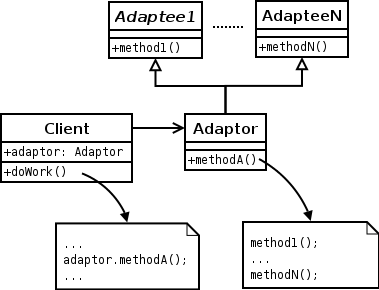
\includegraphics[width=9cm]{figures/adapter.png}
	\caption{Adapter Pattern}
\end{figure}

	\subsection{Observer Pattern}
	
The observer pattern is a software design pattern in which an object, called the subject, maintains a list of its dependents, called observers, and notifies them automatically of any state changes, usually by calling one of their methods.

\begin{figure}[!h]
	\center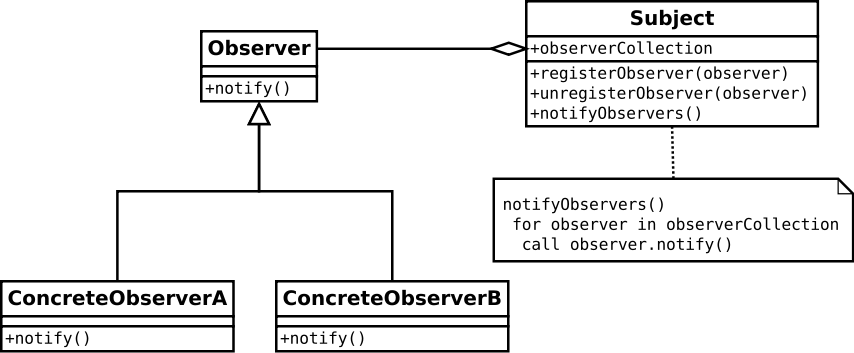
\includegraphics[width=12cm]{figures/observer.png}
	\caption{Observer Pattern}
\end{figure}

\end{document}





